%=====================================================================
%  MODELO DE ARTÍCULO / MONOGRAFÍA — MECÁNICA CUÁNTICA
%  Plantilla elegante en LaTeX  ·  compílese con pdfLaTeX
%  Secuencia:  pdflatex → bibtex → pdflatex → pdflatex
%---------------------------------------------------------------------
%  Autor de la plantilla: (adáptese libremente)
%  Diseño: paleta cálida "Navajo" · tipografía Palatino (mathpazo)
%=====================================================================

\documentclass[11pt,letterpaper]{article}

%========================  CODIFICACIÓN E IDIOMA  =====================
\usepackage[T1]{fontenc}
\usepackage[utf8]{inputenc}
\usepackage{babel}
\babelprovide[import,main]{spanish}          % locale español (babel moderno)

%========================  MATEMÁTICAS Y FUENTE  =====================
\usepackage{amsmath,amssymb}
\usepackage{bm}
\usepackage[sc]{mathpazo}     % Palatino: elegante y muy legible en física
\linespread{1.05}             % interlineado ligeramente holgado
\usepackage{microtype}        % micro-tipografía: mejor gris de página

%========================  GEOMETRÍA Y FIGURAS  ======================
\usepackage[letterpaper,left=2.0cm,right=2.0cm,top=2.0cm,bottom=2.0cm]{geometry}
\usepackage{graphicx}
\usepackage{float}
\usepackage{booktabs}         % reglas de tabla profesionales

%========================  PALETA DE COLOR (navajo_seq)  =============
\usepackage{xcolor}
% Diez tonos del colormap secuencial navajo_seq (frío -> cálido):
\definecolor{navaMidnight}{HTML}{0D1B2A}  % azul noche
\definecolor{navaDeep}{HTML}{1B3A4B}      % pizarra profunda
\definecolor{navaBlue}{HTML}{2E6E8E}      % azul-petróleo
\definecolor{navaTurq}{HTML}{4FA8B8}      % turquesa
\definecolor{navaAqua}{HTML}{88C9C8}      % aguamarina claro
\definecolor{navaCream}{HTML}{F2E8D0}     % crema
\definecolor{navaSand}{HTML}{E8A87C}      % arena / terracota clara
\definecolor{navaBurnt}{HTML}{C46D3B}     % naranja quemado
\definecolor{navaBrick}{HTML}{A0372A}     % ladrillo
\definecolor{navaMaroon}{HTML}{6B1E1E}    % granate oscuro
% Roles del documento (cálidos = jerarquía; frío = enlaces externos):
\colorlet{siena}{navaMaroon}     % títulos de sección, etiqueta Resumen, pies
\colorlet{terracota}{navaBrick}  % subsecciones, enlaces internos, recuadros
\colorlet{ocre}{navaBurnt}       % reglas de acento (portada y secciones)
\colorlet{turquesa}{navaBlue}    % citas y URLs
\colorlet{adobe}{navaSand}       % filetes suaves del resumen
\colorlet{crema}{navaCream}      % fondos de recuadro

%========================  TÍTULOS DE SECCIÓN  =======================
\usepackage{titlesec}
\titleformat{\section}[hang]
  {\normalfont\large\bfseries\color{navaDeep}}
  {\thesection}{0.7em}{}
  [{\vspace{2pt}\color{ocre}\titlerule[0.8pt]}]
\titleformat{\subsection}[hang]
  {\normalfont\normalsize\bfseries\color{navaBlue}}
  {\thesubsection}{0.6em}{}
\titlespacing*{\section}{0pt}{1.6em}{0.7em}
\titlespacing*{\subsection}{0pt}{1.1em}{0.4em}

%========================  PIES DE FIGURA / TABLA  ===================
\usepackage{caption}
\captionsetup{font=small,labelsep=period,labelfont={bf,color=siena}}

%========================  BIBLIOGRAFÍA (natbib)  ====================
\usepackage[numbers,sort&compress]{natbib}
\bibpunct{[}{]}{,}{n}{}{,}

%========================  RECUADROS DE CONSEJO  =====================
\usepackage[most]{tcolorbox}
\newtcolorbox{consejo}{
  enhanced, breakable,
  colback=crema, colframe=terracota,
  boxrule=0.4pt, arc=2.5pt, outer arc=2.5pt,
  left=10pt, right=10pt, top=8pt, bottom=8pt,
  fontupper=\small,
  coltitle=white, colbacktitle=terracota,
  fonttitle=\bfseries\small,
  title=Consejo de redacción,
  attach boxed title to top left={xshift=10pt, yshift=-\tcboxedtitleheight/2},
  boxed title style={boxrule=0pt, arc=2pt},
  top=12pt
}

%========================  OPERADORES Y ATAJOS  ======================
\DeclareMathOperator{\sech}{sech}
\newcommand{\ii}{\mathrm{i}}          % unidad imaginaria
\newcommand{\dd}{\mathrm{d}}          % diferencial recto
\newcommand{\vc}[1]{\bm{#1}}          % vectores en negrita
\newcommand{\op}[1]{\hat{#1}}         % operadores con sombrero

%========================  HIPERVÍNCULOS  ============================
\usepackage[unicode=true,pdfusetitle,colorlinks=true,
            bookmarks=true,pdfborder={0 0 0}]{hyperref}
\hypersetup{linkcolor=terracota, citecolor=turquesa, urlcolor=turquesa}

%---------------------------------------------------------------------
%  Datos del trabajo
%---------------------------------------------------------------------
\newcommand{\subtitulo}{Subtítulo opcional del trabajo}
\title{Título del trabajo}
\author{Nombre del Estudiante}
\date{\today}

\begin{document}

%=====================================================================
%  PORTADA
%=====================================================================
\begin{center}
  {\color{ocre}\rule{0.5\textwidth}{0.8pt}}\\[1.1em]
  {\LARGE\bfseries\color{navaMidnight} Título del trabajo}\\[0.45em]
  {\large\itshape \subtitulo}\\[1.2em]
  {\scshape\large Nombre del Estudiante}\\[0.35em]
  {\small Curso de Introducción a la Física Atómica y Molecular\ \textperiodcentered\ Facultad de Ciencias, UNAM\\
   \texttt{correo@ejemplo.unam.mx}}\\[0.5em]
  {\small \today}\\[0.6em]
  {\color{ocre}\rule{0.5\textwidth}{0.8pt}}
\end{center}
\vspace{0.6em}

%=====================================================================
%  RESUMEN
%=====================================================================
\begin{center}
\begin{minipage}{0.88\textwidth}
  {\color{adobe}\rule{\linewidth}{0.6pt}}\par\vspace{0.6em}
  \small
  \noindent{\bfseries\color{siena} Resumen.\ }%
  El resumen (o \textit{abstract}) es la puerta de entrada al trabajo y, con
  frecuencia, lo único que un lector examina antes de decidir si continúa; por
  ello merece un cuidado especial. Debe ofrecer una descripción concreta y
  autocontenida del problema abordado, de modo que cualquier lector con
  formación en física, aunque no sea especialista en el tema, pueda situarse sin
  recurrir al cuerpo del texto. Se redacta habitualmente en pasado, reservando el
  presente para las afirmaciones de carácter general y para el enunciado de las
  conclusiones. Un buen resumen expone en pocas frases el objetivo principal y su
  alcance, esboza la metodología empleada y anticipa de forma sucinta los
  resultados y la conclusión que se desarrollarán en el cuerpo principal. Conviene
  evitar que resulte extenso o que incorpore detalles técnicos, referencias o
  ecuaciones que solo cobran sentido dentro del texto.
  \par\vspace{0.7em}
  \noindent{\footnotesize\itshape Palabras clave:\/} ejemplo, plantilla, mecánica
  cuántica.
  \par\vspace{0.6em}
  {\color{adobe}\rule{\linewidth}{0.6pt}}
\end{minipage}
\end{center}
\vspace{1.2em}

%=====================================================================
%  INTRODUCCIÓN
%=====================================================================
\section{Introducción}\label{sec:introduccion}

No existe una única forma de redactar una \textit{introducción}: su estilo depende
tanto de la revista o del contexto académico como de la naturaleza de las ideas que
se quieren exponer. Su función, en cambio, es siempre la misma: servir de preámbulo
y ubicar al lector en el marco conceptual donde se desarrolla el tema. En ella se
sintetiza el problema central, a menudo mediante una pregunta que no necesariamente
aparece de forma explícita, y se traza el camino que conducirá a su tratamiento. En
física es habitual que la introducción incluya un breve estado del arte: un recorrido
por los antecedentes y los trabajos previos más relevantes, con sus referencias
correspondientes, que permita delimitar qué aspectos ya están resueltos y cuáles
constituyen el objeto de estudio.

Además de contextualizar, la introducción debe plantear con claridad el problema,
formular la pregunta que se busca responder y enunciar el objetivo del trabajo.
Conviene también anticipar, de manera general, cómo se abordará esa pregunta y qué
tipo de solución se propone; ello prepara al lector para la estructura y la secuencia
en que se desplegarán las ideas. Es costumbre, y una buena práctica, cerrar la
introducción con un párrafo que describa la organización del escrito, resaltando el
objetivo del estudio y ofreciendo una hoja de ruta de las secciones que siguen.

\begin{consejo}
Piense la introducción como un embudo: comience por lo general, el área y su
importancia, y estreche progresivamente hacia lo particular, es decir, su pregunta concreta y
su objetivo. El lector debe llegar al final de esta sección sabiendo \emph{qué} se
investiga, \emph{por qué} importa y \emph{cómo} se ordenará el resto del texto.
\end{consejo}

%=====================================================================
%  DESARROLLO Y MÉTODOS
%=====================================================================
\section{Desarrollo y métodos}\label{sec:desarrollo}

Esta parte constituye el núcleo expositivo del trabajo y, según el problema concreto,
puede dividirse en varias secciones, por ejemplo, para separar el marco teórico de
los métodos experimentales o numéricos. Su rasgo distintivo es la claridad: no solo en
la explicación de los conceptos, sino también en el orden lógico y progresivo con que
se presentan. Aquí las ideas se despliegan de forma ordenada y detallada, y es en este
punto donde el lector debe fijar las nociones fundamentales del tema. A continuación se
ilustran algunos elementos básicos de la escritura en \LaTeX{} de uso frecuente en un
texto de física.

\subsection{La ecuación de Schrödinger}\label{subsec:dinamica}

Consideremos un Hamiltoniano de la forma
\begin{equation}
  \op{H} = -\frac{\hbar^{2}}{2m}\,\nabla^{2} + \op{V}(\vc{r},t),
  \label{eq:hamiltoniano-1}
\end{equation}
que ejemplifica la manera básica de escribir una ecuación numerada. Con él, la
ecuación de Schrödinger dependiente del tiempo~\cite{Shankar-book1994} se expresa como
\[
  \op{H}\,\psi(\vc{r},t) = \ii\hbar\,\dot{\psi}(\vc{r},t),
\]
donde, a diferencia de la anterior, esta ecuación se ha escrito sin numeración.

Las tablas se construyen con el entorno \texttt{tabular}, como se muestra en el
Cuadro~\ref{tab:muestra}.

\begin{table}[h]
  \centering
  \begin{tabular}{ll}
    \toprule
    Columna 1 & Columna 2 \\
    \midrule
    $\alpha$                    & $\beta$ \\
    $\Gamma_{i \rightarrow j}$  & Texto   \\
    \bottomrule
  \end{tabular}
  \caption{Descripción de la tabla.}
  \label{tab:muestra}
\end{table}

De forma análoga, las figuras se insertan con el entorno \texttt{figure};
véase la Fig.~\ref{fig:muestra}.

\begin{figure}[h]
  \centering
  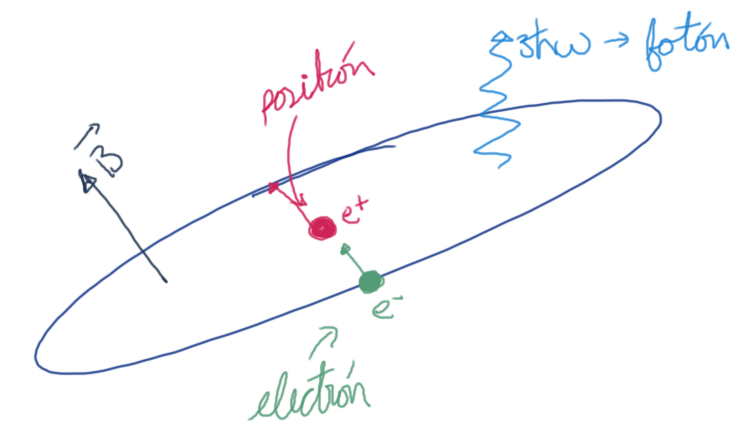
\includegraphics[width=0.68\linewidth]{figuramodelo.png}
  \caption{Esquema de la aniquilación de un par electrón–positrón, con la emisión de
  un fotón de energía $\hbar\omega$, en presencia de un campo magnético externo
  $\vc{B}$.}
  \label{fig:muestra}
\end{figure}

\subsection{Segunda cuantización}\label{subsec:segundacuantizacion}

En la segunda cuantización sustituimos la descripción en términos de partículas por
una en términos de campos, lo que permite distinguir de forma natural entre las
distintas estadísticas~\cite{Pauli-pr58}. Los operadores de campo
$\op{\psi}(\vc{r},t)$ y $\op{\psi}^{\dagger}(\vc{r},t)$ satisfacen, en el caso
bosónico, las relaciones de conmutación
\begin{eqnarray}
  \left[\op{\psi}(\vc{r},t),\op{\psi}^{\dagger}(\vc{r}',t)\right]_{-}
    & = & \delta^{3}(\vc{r}-\vc{r}'), \nonumber \\
  \left[\op{\psi}(\vc{r},t),\op{\psi}(\vc{r}',t)\right]_{-}
    & = & 0, \label{eq:conmutacion} \\
  \left[\op{\psi}^{\dagger}(\vc{r},t),\op{\psi}^{\dagger}(\vc{r}',t)\right]_{-}
    & = & 0. \nonumber
\end{eqnarray}
El subíndice $-$ denota el conmutador,
$[\op{\Omega},\op{\Lambda}]_{-} = \op{\Omega}\op{\Lambda} - \op{\Lambda}\op{\Omega}$;
su anulación en la segunda y tercera líneas refleja la estadística de Bose–Einstein.
Nótese, de paso, cómo se intercalan ecuaciones en el propio texto: los campos
$\op{\psi}(\vc{r},t)$ y $\op{\psi}^{\dagger}(\vc{r},t)$ actúan, respectivamente, como
operadores de aniquilación y de creación. En este formalismo, el Hamiltoniano adopta
la forma
\begin{equation}
  \op{H} = \int \dd^{3}r\;\op{\psi}^{\dagger}(\vc{r},t)
  \left\{ -\frac{\hbar^{2}}{2m}\nabla^{2} + V(\vc{r},t) \right\}
  \op{\psi}(\vc{r},t),
  \label{eq:hamiltoniano}
\end{equation}
es decir, expresado íntegramente en términos de los operadores de campo.

%=====================================================================
%  CITACIONES Y REFERENCIAS
%=====================================================================
\section{Sobre las citaciones y las referencias}\label{sec:citas}

Conviene recordar que toda figura y toda tabla deben estar referenciadas en el cuerpo
del texto; las ecuaciones, en cambio, no requieren mención explícita, aunque
numerarlas resulta siempre útil para las discusiones y para lecturas posteriores. Las
referencias pueden escribirse ``a mano'' o gestionarse con una herramienta como
\textsc{Bib}\TeX{}. Para citar una fuente basta el comando \texttt{\textbackslash cite},
como en~\cite{Pauli-pr58,Shankar-book1994}. Cuando una figura o una tabla se toma de la
literatura, es \textbf{imprescindible} acompañarla de la referencia correspondiente.

El comando \texttt{\textbackslash ref} permite remitir a los distintos elementos del
texto: a ecuaciones —ecs.~(\ref{eq:conmutacion}) y~(\ref{eq:hamiltoniano})—, a
secciones —\S\ref{sec:desarrollo} y~\S\ref{subsec:dinamica}—, a los apéndices
—Ap.~\ref{app:secante}— y a los cuadros —Cuadro~\ref{tab:muestra}. El uso sistemático
de etiquetas (\texttt{\textbackslash label}) y referencias cruzadas mantiene la
numeración coherente aunque el documento se reorganice.

%=====================================================================
%  DISCUSIÓN Y RESULTADOS
%=====================================================================
\section{Discusión y resultados}\label{sec:resultados}

La discusión y los resultados suelen presentarse por separado, pues responden a
propósitos distintos, y habitualmente se redactan en tiempo presente. Es, con
frecuencia, la parte más exigente de elaborar, por su estructura compacta y
organizada. En los resultados se exponen los hallazgos y las soluciones obtenidas
mediante la metodología descrita; en la discusión se retoma la pregunta planteada en la
introducción y se interpreta el significado de esos hallazgos. Se contrasta entonces la
evidencia con los argumentos que sostienen las ideas propuestas, dentro de un marco
lógico y coherente, las mismas ideas que se anticiparon de forma sucinta en la
introducción y se desarrollaron con detalle en el cuerpo del texto.

Esta sección admite cierta libertad interpretativa, siempre dentro del rigor
científico, para destacar la relevancia de los resultados. En ella caben comparaciones
explícitas con otros modelos, teorías o experimentos, así como una valoración de las
ventajas y las limitaciones de la metodología empleada. También es el lugar apropiado
para comentar resultados parciales o anómalos, poco frecuentes o no reportados, y para
proponer explicaciones plausibles de los resultados ``negativos'' o poco concluyentes.
En conjunto, esta parte debe transmitir que las ideas quedan esclarecidas y que se ha
valorado críticamente el alcance de todo lo anterior.

%=====================================================================
%  CONCLUSIONES
%=====================================================================
\section{Conclusiones}\label{sec:conclusiones}

En las conclusiones se cierra el desarrollo del tema y se extraen las consecuencias del
trabajo, sin perder de vista los objetivos, las ideas y la metodología que los
articularon. Conviene subrayar una advertencia habitual: en el ámbito científico, las
conclusiones no son un resumen del texto, aunque exista la tendencia a redactarlas así.
Su cometido es distinto: sintetizar lo aprendido y, cuando resulte pertinente, señalar
los nuevos alcances del trabajo mediante propuestas, sugerencias o recomendaciones que
abran la puerta a investigaciones futuras.

%=====================================================================
%  APÉNDICES
%=====================================================================
\appendix
\section{Apéndices}\label{app:apendices}

Los apéndices permiten incluir desarrollos más detallados o aclarar cálculos que, de
figurar en el cuerpo principal, interrumpirían el hilo de la exposición.

\subsection{Secante hiperbólico}\label{app:secante}

Nótese que en los apéndices también pueden numerarse ecuaciones:
\begin{equation}
  f(x) = \sech^{2}(x).
\end{equation}

%=====================================================================
%  BIBLIOGRAFÍA
%=====================================================================
\bibliographystyle{unsrtnat}   % numérica, en orden de aparición (estilo físico)
\bibliography{modelobib}

\end{document}
